%!TEX root = thesis.tex

\chapter{Implementation of OTM over the FFI}

\label{chap:implementation}
\begin{wrapfigure}{r}{0.27\textwidth}
\vspace{-30pt}
\centering
    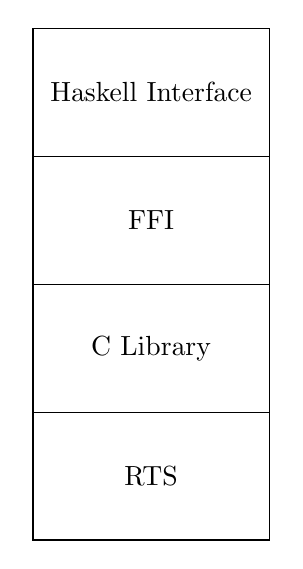
\begin{tikzpicture}[
            lbl/.style={
              text width=2.9cm,
              align=center
            }
        ]
    \def\h{6.5cm}
    \draw (0,0) rectangle (3,\h) {};

    \foreach \i in {1,2,3}
      \draw (0,{\i*\h/4}) -- +(3,0) {};

    \foreach \i/\n in {0/RTS, 1/C Library, 2/FFI, 3/Haskell Interface}
        \node[lbl] at (1.5,{\h/8 + \i*\h/4}) {\n};

    \end{tikzpicture}
    \caption{Library overview}
\end{wrapfigure}

In this chapter we present the most important parts of our implementation.
At a high level the implementation is subdivided in an Haskell library and a C library.
The data structures, as well as the operations on them, are defined in the C Header file OTM.h and made available to the Haskell code through the Foreign Function Interface.
Since the FFI does not provide a type safe marshaling for pointers, we decided to introduce the C2HS preprocessor to our build scheme.
All the foreign declarations reside in the file Internals.chs and are written with the syntax of C2HS.\cite{Chakravarty2000}
Finally the OTM interface shown in \cref{fig:base-interface} is exposed by the the Haskell module Control.Monad.OTM and defined in the file OTM.hs.

\begin{figure}[b]
\vspace{-14pt}
\begin{lstlisting}[language=Haskell]
type TM = StateT OTRec (ExceptT RetryException IO)

newtype OTM a = OTM { unOTM :: TM a }
    deriving (Functor, Applicative, Monad)

newtype ITM a = ITM { unITM :: TM a }
    deriving (Functor, Applicative, Monad)

evalOTM :: OTM a -> OTRec -> IO (Either RetryException a)
evalOTM otm s = runExceptT . flip evalStateT s $ unOTM otm

evalITM :: ITM a -> OTRec -> IO (Either RetryException a)
evalITM itm s = runExceptT . flip evalStateT s $ unITM itm
\end{lstlisting}
\caption{Monads of the OTM library}
\label{fig:monads}
\end{figure}

\section{Monads TM, OTM and ITM}
The \emph{TM Monad} is at the hearth of our transactional memory implementation;
as shown in \cref{fig:monads}, the monads OTM and ITM are \emph{newtype} declarations that encapsulate a value of type \emph{TM a}.
The \emph{TM Monad} is a type synonym for a stack of monad transformers that solve the following constraints:
\begin{itemize}
\item reads and writes are foreign functions with side effects, thus the IO monad is the innermost;
\item transactions may explicitly fail, \ie, call \emph{retry}, thus the \emph{ExceptT} monad transformer allows computations to terminate with an exceptional value;
\item transactions need to keep track of their state, reads and tentative writes, thus the \emph{StateT} monad transformer adds a transactional log as the state of the computation.

\end{itemize}
\section{Transactional record and OTVars}
\begin{figure}[t]
\begin{lstlisting}
-- Transactional record for Haskell code
newtype OTRec = OTRec (ForeignPtr OTRec)

-- Transactional variable for Haskell code
newtype OTVar a = OTVar (ForeignPtr (OTVar a))

-- Transactional record for C code
struct OTRecHeader_ {
    struct OTRecHeader_ *enclosing_trec;        // Used by nested transactions
    OTRecNode           *volatile forward_trec; // Union-Find information
    OTRecChunk          *current_chunk;         // Array of OTRecEntries
    OTRecState           volatile state;        // State of the transaction
    Cond                 condition_variable;    // Used by retry mechanism
};

-- Transactional variable for C code
typedef struct {
    OtmStablePtr     volatile current_value;            // Current value
    OTVarWatchQueue *volatile first_watch_queue_entry;  // Wait queue
    HsWord           volatile locked;                   // 0 means not locked
    OTVarDelta      *volatile delta;                    // Shared memory
} OTVar;
\end{lstlisting}
\caption{Data structures}
\vspace{-8pt}
\end{figure}
The transactional record (\emph{OTRec}) contains an entry for each \emph{OTVar} that the transaction has accessed.
Each entry in the transactional log is an \emph{OTRecEntry} that contains a reference to the \emph{OTVar} involved and two additional fields used only by \emph{Isolated Transaction}.
This additional fields, that contain the \emph{old value} held in the \emph{OTVar} when it was first accessed and the \emph{new value} to be committed if the validation succeeds, represent the working memory of an isolated transaction.

The accesses to OTVars performed by isolated transactions remain buffered within the transactional record and invisible to other threads until the transaction commit. \emph{Open Transactions}, instead, perform this accesses in a shared working memory, that we call \emph{OTVarDelta} or \emph{delta memory}, retained directly by the \emph{OTVar}.

Both \emph{OTVar} and \emph{OTRecEntry}, hold pointers to Haskell values.
As explained in \cref{ffi:stableptr}, this pointers must be \emph{Stable Pointers}: when we write a value in an \emph{OTVar}, this value is wrapped inside a \emph{StablePtr}.
The same stable pointer could be copied in the working memory of several transactions, so reference counting is added to each pointer: when there are no more references left to a pointer, \emph{freeStablePtr} is called.

The transactional record contains additional informations that describe the state of the transaction, \ie, in which phase of the life cycle it is, the number of total threads participating to this transaction and the number of threads that are still running.

The \emph{OTRec} and the \emph{OTVar} are allocated by the foreign code, but wrapped inside a \emph{Foreign Pointer} so their life span is managed by the garbage collector.

\section{Transaction life-cycle}

The life-cycle of an \emph{Open Transaction} is quite complex compared to that of an \emph{Isolated Transactions}, which will be omitted.

The life-cycle of an open transaction is summarized by the automaton in \cref{fig:implementation-lifecycle}.
In this automaton, each transition is labeled with a triple ``a;c;v'' where \emph{a} is the action (possibly with parameters), \emph{c} is a condition under which the action can be taken, and \emph{v} is the list of new values to put in the target state registers.

The state of a running transaction is \emph{Ru\textlangle n, l\textrangle}, where \emph{n} is the number of threads that have not already voted to commit, and \emph{l} is the total number of threads participating to the transaction.
This is the only state where new threads can be merged to the transaction. When a transaction is created, its state is \emph{Ru\textlangle 1, 1\textrangle}.
When another transaction is merged, we add the registers componentwise; when a thread returns and hence is ready to commit, \emph{n} is decremented.
If it is the one that zeros \emph{n}, the transaction is ready to commit: its state changes to \emph{Co\textlangle l, l\textrangle} , where every participant commits and decrements \emph{n}; eventually, we conclude the transaction by moving to state \emph{Co!\textlangle \textrangle}.
If a thread executes a retry, the transaction moves immediately to state \emph{Re\textlangle l, l\textrangle} and waits that every other participant acknowledges the retry, decrementing \emph{n}, before restarting the transaction.
The abort procedure (initiated by a throw) is analogous, apart from the fact that we have to propagate the exception \emph{e}.
The states \emph{Co!\textlangle \textrangle }, \emph{Ab!\textlangle e\textrangle}  and \emph{Re!\textlangle \textrangle}  identify the states of the machine when \emph{n} = 0 and the commit, abort or retry procedures are completed, respectively.
\begin{figure*}
    \centering
    \begin{tikzpicture}[
            font=\small,
            state/.style={
                draw=black,fill=white,align=center,
                outer sep=0pt,
                inner sep=5pt,
                rounded corners=3pt,
            },
            lbl/.style={align=center},
            trs/.style={->,>=stealth',shorten >=1pt},
        ]

        \coordinate (S) at (-4.8,2.8);
        \node[state] (Ru) at (-2,1.7) {Ru$\langle n, l\rangle$};
        \node[state] (Co) at (3,3.4) {Co$\langle n, l\rangle$};
        \node[state] (Re) at (3,1.7) {Re$\langle n, l\rangle$};
        \node[state] (Ab) at (3,0) {Ab$\langle n, l, e\rangle$};
        \node[state] (CoT) at (8,3.4) {Co!$\langle\rangle$};
        \node[state] (ReT) at (8,1.7) {Re!$\langle\rangle$};
        \node[state] (AbT) at (8,0) {Ab!$\langle e \rangle$};
%        \coordinate (CoT) at (5.5,4.7);
%        \coordinate (ReT) at (5.5,2.5);
%        \coordinate (AbT) at (5.5,0.3);

        \draw[trs] (S) to node[lbl,anchor=north east,pos=.3]
            {new; $\top$; $\langle 0,1 \rangle$} (Ru.north west);

        \draw[trs,loop below] (Ru) to node[lbl,below left]
            {merge ${\langle n', l'\rangle}$; $\top$; $\langle n + n', l + l' \rangle$} (Ru);
        \draw[trs,loop left,] (Ru) to node[lbl,below left]
            {fork; $\top$; $\langle n,l+1 \rangle$} (Ru);
        \draw[trs,loop above] (Ru) to node[lbl,above]
            {return; $n-1>0$; $\langle n-1,l \rangle$} (Ru);

        \draw[trs] (Ru) to node[lbl,anchor=south east, pos=.95]
            {return; $n-1=0$; $\langle l,l \rangle$} (Co.west);
        \draw[trs] (Ru) to node[lbl,anchor=south east, pos=.95]
            {retry; $\top$; $\langle l,l \rangle$} (Re.west);
        \draw[trs] (Ru) to node[lbl,anchor=north east, pos=.95]
            {throw $e$; $\top$; $\langle l, l, e \rangle$} (Ab.west);

        \draw[trs,loop above] (Co) to node[lbl,above]
            {commit; $n-1>0$; $\langle n-1,l \rangle$} (Co);
        \draw[trs,loop above] (Re) to node[lbl,above]
            {restart; $n-1>0$; $\langle n-1,l \rangle$} (Re);
        \draw[trs,loop above] (Ab) to node[lbl,above]
            {abort; $n-1>0$; $\langle n-1, l, e \rangle$} (Ab);

        \draw[trs] (Co) to node[lbl,above]
            {commit; $n-1=0$; $\langle\rangle$} (CoT);
        \draw[trs] (Re) to node[lbl,above]
            {restart; $n-1=0$; $\langle\rangle$} (ReT);
        \draw[trs] (Ab) to node[lbl,above]
            {abort; $n-1=0$; $\langle e \rangle$} (AbT);
    \end{tikzpicture}
    \caption{Transaction life-cycle.}
    \label{fig:implementation-lifecycle}
\end{figure*}

\section{Validation and commit}

Both \emph{atomic} and \emph{isolated} functions operate by executing the computation of type \emph{TM a} encapsulated inside a monadic value of type \emph{OTM a} and \emph{ITM a} by means the functions declared in \cref{fig:monads}; the validation phase is where the two functions differ.

% \begin{figure}
% \begin{lstlisting}[language=Haskell,showlines=false]
% otmCommit :: OTRec -> IO OTState
% otmRetry  :: OTRec -> IO OTState
% otmAbort  :: OTRec -> StablePtr SomeException -> IO OTState
% \end{lstlisting}
% \caption{Agreement interface}
% \label{fig:agreement}
% \end{figure}

\begin{figure}
\begin{lstlisting}[language=Haskell]
atomic:: forall a . OTM a -> IO a
atomic otm = do
    otrec <- startOpenTransaction
    result <- try $ evalOTM otm otrec
    case result of
        Left se -> do
            exp <- newStablePtr se
            state <- otmAbort otrec exp
            otmHandleTransaction otrec otm state
        Right computation ->  case computation of
            Left _ -> do
                state <- otmRetry otrec
                otmHandleTransaction otrec otm state
            Right v -> do
                state <- otmCommit otrec
                case state of
                    OtrecCommited -> return v
                    _ -> otmHandleTransaction otrec otm state
\end{lstlisting}
\caption{\emph{atomic} implementation}
\label{fig:atomic}
\end{figure}

In the case of an \emph{Open Transaction}, the \emph{validation process} consists of two phases: a \emph{voting phase} and an \emph{agreement phase}.
Each thread participating in a transaction, checks the value returned by the executed computation and vote accordingly to change the transaction state.
\newpage
The vote is expressed by means the functions:
% in \cref{fig:agreement},
\begin{lstlisting}[language=Haskell,showlines=false]
otmCommit :: OTRec -> IO OTState
otmRetry  :: OTRec -> IO OTState
otmAbort  :: OTRec -> StablePtr SomeException -> IO OTState
\end{lstlisting}
which initiate the \emph{validation phase} for the current thread.

Regarding \cref{fig:atomic}, if the transactional computation of type \emph{OTM a} ends without exceptional values, the thread calls \emph{otmCommit}: this foreign function decrements the counter of running threads, and sleeps as long as the state of the transaction remain \emph{Ru\textlangle \_,\_\textrangle}, waiting the vote of the other participating threads.
When the state changes, it means that the transaction's \emph{voting phase} ended and the threads have agreed on one of the states \emph{Co\textlangle n, l\textrangle}, \emph{Re\textlangle n, l\textrangle} or \emph{Ab\textlangle n, l\textrangle}.
If the new state is \emph{Co\textlangle n, l\textrangle}, the transaction initiate the \emph{committing phase} and the value \emph{n} represents the number of threads that have to commit their working memory.
Each thread updates the \emph{current value} of the \emph{OTVars} in its transactional record with the value held by the \emph{delta memory}. When a thread updates all the variables in its transactional log, it acknowledges the transaction decrementing the number of \emph{committing threads}.
If the \emph{agreed} state is one of \emph{Re\textlangle n, l\textrangle} and \emph{Ab\textlangle n, l\textrangle} the transactional record is discarded, the threads disjointed, and the transaction re-executed. The re-execution of a transaction is managed by the function:
\begin{lstlisting}
otmHandleTransaction:: OTRec -> OTM a -> OTState -> IO a
\end{lstlisting}

If an exceptional value of type \emph{RetryException} is returned by the OTM computation, the thread calls \emph{otmRetry} to move the transaction in the state \emph{Re\textlangle l,l\textrangle} and wait that the other threads acknowledge and agree on the new state. If other exceptions are caught, \emph{otmAbort} is called, and the exception is propagated outside the transaction. If a transaction aborts or retries, all the threads retry the execution with a fresh transactional log, except the one that threw the exception.

%To summarize, the validation phase of an \emph{Open Transaction} is an agreement phase between the participating threads.

Different is the validation of an \emph{Isolated Transaction}.
In the validation phase of these transactions, each \emph{OTVar} in the transactional log is locked and the expected value held in the \emph{OTRecEntry} is compared with the \emph{OTVar}'s \emph{shared value}.
The lock is a tentative lock, so either is not acquired or the shared value is different from the expected one, the transaction validation fails.
If the validation succeeds, the writes in the log are made visible to other threads committing the changes in the OTVars shared memory. Since an isolated transaction is nested inside an open transaction, the commit of an isolated transaction can trigger merges between open transactions.

\section{Merge of transactions}

Transaction merging is triggered by operations on the shared memory.
This operations are reads and writes of \emph{OTVar}s in the OTM monad, and commits of isolated transactions.

\begin{figure}
\begin{lstlisting}
-- Haskell declaration
otmReadOTVar :: OTRec -> OTVar a -> IO (StablePtr a)

-- C declaration
HsStablePtr otmReadOTVar(OTRecHeader* trec, OTVar* otvar) {
    TRACE("trec: %p read  %p", trec, otvar);
    assert(trec -> forward_trec != NULL);

    if(!otm_acquire_OTVar_read(trec, otvar)) {
        if(!otmUnion(trec, otvar -> delta -> trec)){
            // Retry the read
            // otvar's trec is OTREC_ABORTED || OTREC_COMMITED || OTREC_RETRYED
            return otmReadOTVar(trec, otvar);
        }
    }
    while(otvar -> locked) {    // An isolated transaction is committing
        busy_wait_nop();
    }
    return otvar -> delta -> new_value -> ptr;
}
\end{lstlisting}
\caption{Open read of an OTVar}
\label{fig:otmread}
\vspace{-5pt}
\end{figure}

The first time an \emph{OTVar} is accessed, it is \emph{acquired} by the transaction that requested the operation: its \emph{delta memory}, initially empty, is filled in with an \emph{OTVarDelta} containing the \emph{shared value} and a reference to the transaction which is acquiring the variable.
As shown in \cref{fig:otmread} line 9, the \emph{acquiring phase} is the first phase of a read or a write in the OTM monad.
This phase is a tentative update of the \emph{delta memory} of an \emph{OTVar} carried out atomically by means a \emph{compare\&swap} instruction: if it fails, the \emph{OTVar}'s \emph{delta memory} was not empty, thus the variable had already been acquired by another transaction.

\begin{figure}
\begin{lstlisting}[language=C]
HsBool otmUnion(OTRecHeader* trec1, OTRecHeader* trec2){
    OTRecHeader *x, *y, *temp;
    OTState x_s, y_s;
    HsWord x_rank, y_rank, t_rank;
    HsBool result;
    do {
        // Find the roots of the Union-Find
        x = find(trec1);
        y = find(trec2);
        if (x == y) {
            return TRUE;
        }
        if (is_greater_then(x, y)) {
            temp = x;
            x = y;
            y = temp;
        }
        // Invariant x < y
        x_rank = x -> forward_trec -> rank;
        y_rank = y -> forward_trec -> rank;
        x_s = lock_OTRec(x);
        y_s = lock_OTRec(y);
        if (!((x_s & y_s) & OTREC_RUNNING)) {
            // If both transaction are not running
            unlock_OTRec(y, y_s);
            unlock_OTRec(x, x_s);
            return FALSE;
        }
        result = update_root(x, x_rank, y, y_rank);
        if (result) {
            if (x_rank == y_rank) {
                update_root(y, y_rank, y, y_rank +1);
            }
            // Fix (long) equal ranked chains
            setRoot(x);
            y -> state.running += x -> state.running;
            y -> state.threads += x -> state.threads;
        }
        unlock_OTRec(y, y_s);
        unlock_OTRec(x, x_s);
    } while (!result);
    return TRUE;
}
\end{lstlisting}
\caption{Merge of transactions}
\label{fig:otmunion}
\end{figure}

When a transaction reads or writes an owned \emph{OTVar}, the function \emph{otmUnion} is called (\cref{fig:otmread} line 10).
To represent transaction merges we opted for a Union-Find data structure with the heuristics of \emph{path compression} and \emph{union by rank}.
Each transactional record has a \emph{forward transaction} field that stores the information needed by the data structure: the \emph{rank} of that node and a \emph{reference} to the \emph{root} of the set.
We followed the implementation proposed by \citet{Anderson94wait-freeparallel} where operations on the data structure are lock free.
To adapt their implementation to our needs, we introduced the lock of the root nodes involved in the \emph{union} procedure. Unlike a normal Union-Find, when two root nodes are merged, we have to update both: in one the \emph{forward transaction} field and in the other the number of participating threads. This entails the inevitable use of locks.

The \emph{otmUnion} function is shown in \cref{fig:otmunion}. It acquires the locks on the transactional records that have to be merged and performs a union by rank. If the union succeeds, the number of running and participating threads of one transaction is added to that of the new root transaction. The transactional log that is no longer representing a transaction, becomes a mere node of the Union-Find with the unique scope of referencing the root of the set. Attempting to merge transactions that are not in the \emph{Ru\textlangle n, l\textrangle} state, causes the union process failure (lines 23-28).

For the read operation in \cref{fig:otmread}, the success of the \emph{otmUnion} function allows its conclusion by returning the value held in the \emph{OTVar}'s \emph{delta memory}. Instead, a write operation ends by atomically writing the \emph{delta memory} of an OTVar.
